\chapter{休克尔理论与共轭体系}\label{ch:b2:huckel}

向环己烯中加氢，每摩尔放出 \qty{119}{kJ} 热量。苯，
在六个碳组成的环上含三个双键，若在加氢变为环己烷的过程中，
应放出三倍的热量；实际却少放出 \qty{150}{kJ}。这一缺失的
能量即为芳香环的稳定性，它也是苯难以发生烯烃所常见
加成反应的原因。1931 年，埃里希·休克尔用一个
行列式计算了它，做法是把分子简化为其 $\pi$ 电子及其
邻接关系。他的方法虽然粗略，却说明了六个 $\pi$
电子构成的环为何特殊、长共轭链为何吸收可见光，
以及共轭分子的电荷位于何处。

\begin{recall}
\Cref{ch:b2:diatomic-mos}：\omterm{def:b2:diatomic-mos:integrals}{库仑积分} $\alpha$，\omterm{def:b2:diatomic-mos:integrals}{共振积分} $\beta$、
\omterm{def:b2:diatomic-mos:integrals}{久期行列式}。\Cref{ch:b2:fragment-orbitals}：乙烯与烯丙基的 $\pi$ 轨道。
本科一年级分册：共轭体系、共振、发色团和
吸收峰。
\end{recall}

\section{休克尔方法}

在平面共轭分子中，$\sigma$ 轨道关于该平面对称，垂直于平面的 p
轨道关于该平面反对称：二者互不混合
（\cref{prop:b2:diatomic-mos:symmetry}），因而可单独处理 $\pi$
电子。

\begin{definition}[休克尔方法]\label{def:b2:huckel:method}
\emph{休克尔方法}\index{休克尔方法}用以计算平面共轭体系的 $\pi$ 轨道，
即将其表示为每个原子一个 p 轨道的 $\psi = \sum_r c_r p_r$ 形式的线性组合，
并采用以下近似：\omterm{def:b2:diatomic-mos:integrals}{重叠积分} $S_{rs} = 0$（$r \neq s$ 时），$r =
s$ 时为 1；所有\omterm{def:b2:diatomic-mos:integrals}{库仑积分}均取为 $\alpha$；成键近邻之间的\omterm{def:b2:diatomic-mos:integrals}{共振积分}取为 $\beta < 0$，
其余为零。
\end{definition}

令 $x = (\alpha - E)/\beta$，则对每个原子 $r$，久期方程变为
$xc_r + \sum_{s \text{ 键合于 } r} c_s = 0$，
能量即为以 $x$ 为对角元、成键原子间为 1 的行列式的根。等价地，$E =
\alpha + m\beta$，其中 $m$ 为该分子碳骨架邻接矩阵的本征值；
由于 $\beta < 0$，正的 $m$ 对应成键能级。

\begin{method}[休克尔计算]\label{met:b2:huckel:huckel}
\begin{enumerate}
  \item 将共轭原子编号，写出矩阵：对角元为 0，
        成键的每一对原子处为 1。
  \item 求其本征值 $m_k$（用下面的闭合形式或数值方法）：$E_k =
        \alpha + m_k\beta$。
  \item 从最成键的能级起填充电子，每级两个电子：
        $E_\pi = \sum_k n_k E_k$。
  \item 由归一化系数计算电荷与\omterm{def:b2:diatomic-mos:bond-order}{键级}。
\end{enumerate}
\end{method}

\begin{proposition}[迹]\label{prop:b2:huckel:trace}
休克尔体系中 $n$ 个 $\pi$ 轨道的能量之和为 $n\alpha$。
\end{proposition}

\begin{proof}
矩阵本征值之和等于其迹；休克尔矩阵以 $\alpha$ 为
其全部 $n$ 个对角元。
\end{proof}

\section{线性多烯}

\begin{theorem}[线性链的能级]\label{thm:b2:huckel:polyene}
含 $n$ 个原子的线性共轭链具有如下能级与系数：
\[
  E_k = \alpha + 2\beta\cos\frac{k\pi}{n + 1}, \qquad
  c_{jk} = \sqrt{\frac{2}{n + 1}}\,\sin\frac{jk\pi}{n + 1}, \qquad k = 1, \dots, n .
\]
\end{theorem}

\begin{proof}
久期方程为 $c_{j-1} + xc_j + c_{j+1} = 0$，$j = 1, \dots, n$，
且 $c_0 = c_{n+1} = 0$。试取 $c_j = \sin j\theta$：$\sin(j - 1)\theta + \sin(j + 1)\theta = 2\sin
j\theta\cos\theta$，故方程在 $x = -2\cos\theta$ 时成立，且 $c_0 = 0$
自动满足。端点条件 $c_{n+1} = \sin(n + 1)\theta = 0$ 给出 $\theta =
k\pi/(n + 1)$。于是 $E = \alpha - x\beta = \alpha + 2\beta\cos\theta$。归一化时用到
$\sum_{j=1}^n\sin^2 j\theta = (n + 1)/2$。
\end{proof}

\begin{example}[丁二烯]\label{ex:b2:huckel:butadiene}
当 $n = 4$ 时：$E = \alpha \pm 1.618\beta$，$\alpha \pm 0.618\beta$。四个 $\pi$ 电子填充两个
成键能级：$E_\pi = 4\alpha + 2(1.618 + 0.618)\beta = 4\alpha + 4.472\beta$。最低
轨道系数为 0.372、0.602、0.602、0.372，次低轨道为 0.602、0.372，
$-0.372$、$-0.602$。
\end{example}

\begin{omfigure}
\begin{tikzpicture}[font=\small]
  \foreach \k/\a/\b/\c/\d/\lab in {1/0.372/0.602/0.602/0.372/{$\psi_1$, $\alpha + 1.618\beta$},
      2/0.602/0.372/-0.372/-0.602/{$\psi_2$, $\alpha + 0.618\beta$},
      3/0.602/-0.372/-0.372/0.602/{$\psi_3$, $\alpha - 0.618\beta$},
      4/0.372/-0.602/0.602/-0.372/{$\psi_4$, $\alpha - 1.618\beta$}} {
    \begin{scope}[yshift={(\k-1)*2.1cm}]
      \draw[black!40] (-0.2,0) -- (3.2,0);
      \pic at (0,0) {omp={1.6*\a}{90}}; \pic at (1,0) {omp={1.6*\b}{90}};
      \pic at (2,0) {omp={1.6*\c}{90}}; \pic at (3,0) {omp={1.6*\d}{90}};
      \node[anchor=west] at (3.6,0) {\lab};
    \end{scope}
  }
\end{tikzpicture}

{\small 丁二烯的四个 $\pi$ 轨道，波瓣按
休克尔系数（已算出）绘制并按符号着色；能量向上递增，
节点数依次为 $0, 1, 2, 3$。下面两个轨道已被填充。}
\end{omfigure}

\begin{definition}[$\pi$ 电荷与键级]\label{def:b2:huckel:indices}
设 $n_k$ 为轨道 $k$ 中的电子数（取 0、1 或 2），$c_{rk}$ 为实系数，
\emph{$\pi$ 电荷}\index{$\pi$ 电荷}为原子 $r$ 上的 $q_r = \sum_k n_kc_{rk}^2$（即
该原子所带的 $\pi$ 电子数），\emph{$\pi$ 键级}\index{$\pi$ 键级}
键 $rs$ 的\omterm{def:b2:diatomic-mos:bond-order}{键级}为 $p_{rs} = \sum_k n_kc_{rk}c_{sk}$。
\end{definition}

对于丁二烯，$p_{12} = 2(0.372 \times 0.602 + 0.602 \times 0.372) = 0.894$ 与 $p_{23} =
2(0.602^2 - 0.372^2) = 0.447$：两端的键承担了大部分 $\pi$ 成键作用，且
键长较短，中间键具有部分双键性质。所有电荷
均为 1。

\begin{proposition}[交错烃]\label{prop:b2:huckel:alternant}
在中性烃中，若其共轭原子可染成两组，
同一组内任意两个原子互不相邻（无奇数元环），则每个 $\pi$ 电荷都等于 1。
\end{proposition}

\admitted

该结论（库尔森与拉什布鲁克）已在上文丁二烯上检验，在苯上则借助
对称性验证；这也解释了此类烃的
$\pi$ 电子不产生永久偶极矩。

\begin{definition}[离域能]\label{def:b2:huckel:delocalisation}
称共轭体系的\emph{离域能}\index{离域能}
为其 $\pi$ 能量与相同数目
孤立双键的能量之差，每个孤立双键的 $E_\pi = 2\alpha + 2\beta$。
\end{definition}

对于丁二烯，其值为 $4.472\beta - 4\beta = 0.472\beta$；对于己三烯，为 $0.988\beta$。

\section{环与芳香性}

\begin{theorem}[环的能级]\label{thm:b2:huckel:ring}
平面环含 $n$ 个共轭原子，其能级为 $E_k = \alpha + 2\beta\cos(2\pi k/n)$，
$k = 0, 1, \dots, n - 1$：一个最低能级 $\alpha + 2\beta$，其后为成对的简并能级，
若 $n$ 为偶数，则还有一个最高能级 $\alpha - 2\beta$。
\end{theorem}

\begin{proof}
在环中，每个原子有两个近邻，下标按模 $n$ 取值：
有 $c_{j-1} + xc_j + c_{j+1} = 0$（对所有 $j$），且 $c_{j+n} = c_j$。试取 $c_j = \mathrm e^{\mathrm
i jq}$：由方程得 $x = -(\mathrm e^{-\mathrm iq} + \mathrm e^{\mathrm iq}) = -2\cos q$，
且周期性要求 $nq = 2\pi k$。能级 $k$ 与 $n - k$
的能量相同，它们的和与差是实轨道。只有 $k = 0$（以及 $k = n/2$，
$n$ 为偶数时）对应单一能级。
\end{proof}

\begin{corollary}[弗罗斯特圆]\label{cor:b2:huckel:frost}
环的能级可在半径为 $2|\beta|$、以 $\alpha$ 为中心的圆上读出，
其中内接一个正 $n$ 边形，且一个顶点位于底部：每个顶点
的高度即对应一个能级。
\end{corollary}

\begin{proof}
多边形的第 $k$ 个顶点位于角 $-\pi/2 + 2\pi k/n$ 处，其高度为
$-2|\beta|\cos(2\pi k/n) = 2\beta\cos(2\pi k/n)$，相对于中心。
\end{proof}

\begin{omfigure}
\begin{tikzpicture}[font=\scriptsize]
  \foreach \n/\x/\name/\el in {4/0/{\ce{C4H4}}/4, 5/3.4/{\ce{C5H5-}}/6, 6/6.8/{\ce{C6H6}}/6, 7/10.2/{\ce{C7H7+}}/6} {
    \begin{scope}[xshift=\x cm]
      \draw[black!35] (0,0) circle (1.2);
      \draw[black!60] \foreach \k in {0,...,\the\numexpr\n-1\relax} { ({-90+360*\k/\n}:1.2) -- ({-90+360*(\k+1)/\n}:1.2) };
      \foreach \k in {0,...,\the\numexpr\n-1\relax} {
        \draw[very thick] ({1.2*cos(-90+360*\k/\n)-0.22},{1.2*sin(-90+360*\k/\n)}) -- ({1.2*cos(-90+360*\k/\n)+0.22},{1.2*sin(-90+360*\k/\n)});
      }
      \draw[densely dotted] (-1.5,0) -- (1.5,0);
      \node[font=\small] at (0,-1.75) {\name};
    \end{scope}
  }
  \node[anchor=east] at (-1.5,0) {$\alpha$};
  % electrons: C4H4 (2 + 1 + 1), others filled lowest three
  \foreach \x in {0,3.4,6.8,10.2} {
    \draw[-{Stealth[length=1mm]}, thick] ({\x-0.05},-1.32) -- ({\x-0.05},-1.08);
    \draw[-{Stealth[length=1mm]}, thick] ({\x+0.05},-1.08) -- ({\x+0.05},-1.32);
  }
  % six-electron rings: the lowest degenerate pair is filled
  \foreach \n/\x in {5/3.4, 6/6.8, 7/10.2} {
    \foreach \k in {1, \the\numexpr\n-1\relax} {
      \pgfmathsetmacro\ex{\x + 1.2*cos(-90 + 360*\k/\n)}
      \pgfmathsetmacro\ey{1.2*sin(-90 + 360*\k/\n)}
      \draw[-{Stealth[length=1mm]}, thick] ({\ex-0.05},{\ey-0.12}) -- ({\ex-0.05},{\ey+0.12});
      \draw[-{Stealth[length=1mm]}, thick] ({\ex+0.05},{\ey+0.12}) -- ({\ex+0.05},{\ey-0.12});
    }
  }
  % C4H4: one electron in each of the two nonbonding levels
  \draw[-{Stealth[length=1mm]}, thick] (1.2,-0.12) -- (1.2,0.12);
  \draw[-{Stealth[length=1mm]}, thick] (-1.2,-0.12) -- (-1.2,0.12);
\end{tikzpicture}

{\small 弗罗斯特圆。各多边形的顶点（一个位于底部）
内接于半径为 $2|\beta|$ 的圆中，给出该环的能级。当 $\pi$ 电子数为六时，
\ce{C5H5-}、\ce{C6H6} 和 \ce{C7H7+} 填满最低能级及一对简并能级，
形成闭壳层。环丁二烯的四个电子中，有两个电子处于
一对简并\omterm{def:b2:diatomic-mos:bonding}{非键轨道}上（图中已画出）。}
\end{omfigure}

\begin{definition}[芳香性]\label{def:b2:huckel:aromatic}
环状、平面、完全共轭的体系，若其
$\pi$ 电子形成具有较大\omterm{def:b2:huckel:delocalisation}{离域能}的闭壳层，则称其为\emph{芳香性的}\index{芳香性的}，而
若其 $\pi$ 电子半充满一对简并
轨道，则称其为\emph{反芳香性的}\index{反芳香性的}，这使其稳定性低于相应的开链体系。
\end{definition}

\begin{theorem}[休克尔规则]\label{thm:b2:huckel:huckel-rule}
平面单环共轭体系具有 $\pi$ 电子闭壳层，当且仅当
其电子数为 $4N + 2$（$N = 0, 1, 2, \dots$）；若电子数为 $4N$，则
有两个电子处于一对半充满的简并轨道中。这就是\emph{休克尔规则}\index{休克尔规则}。
\end{theorem}

\begin{proof}
由\cref{thm:b2:huckel:ring}可知，自下而上的能级依次为一个单一能级，
其后为成对的简并能级（仅就占据部分而言）。闭壳层填满单一能级
（2 个电子）和整数 $N$ 对简并能级（每对 4 个电子）：$4N + 2$。若电子数为
$4N$，则最后一对只容纳两个电子，各占一个轨道（洪特
规则）。
\end{proof}

\begin{method}[是否芳香？]\label{met:b2:huckel:aromaticity}
\begin{enumerate}
  \item 体系是否为环，且每个原子上都有一个 p 轨道（计入碳正离子
        和碳负离子中心，以及杂原子上的孤电子对）？
  \item 它能否为平面结构？
  \item 数一数 $\pi$ 电子的个数：若为平面结构，则 $4N + 2$ 为芳香性，$4N$ 为反芳香性。
  \item 若可能，反芳香性环应避免平面化或共轭
        （环辛四烯呈盆形，其行为与多烯相似）。
\end{enumerate}
\end{method}

\begin{example}[苯]\label{ex:b2:huckel:benzene}
六个 $\pi$ 电子填入 $\alpha + 2\beta$ 能级及 $\alpha + \beta$ 能级对：$E_\pi = 6\alpha + 8\beta$。
三个孤立双键给出 $6\alpha + 6\beta$：\omterm{def:b2:huckel:delocalisation}{离域能}为 $2\beta$，
约为六碳开链己三烯（$0.988\beta$）的两倍：
闭环所带来的稳定化与之相当。由对称性，所有\omterm{def:b2:diatomic-mos:bond-order}{键级}相等（$p = 2/3$），六个键长
亦相等，均为 \qty{139.7}{pm}，介于乙烯（\qty{133.9}{pm}）与乙烷
（\qty{153.6}{pm}）之间。
% ledger: geo:C6H6.rCC, geo:C2H4.rCC, geo:C2H6.rCC
\end{example}

\begin{omfigure}
\begin{tikzpicture}[font=\small, y=0.013cm, x=1.0cm]
  \draw[thick] (0,0) -- (10.5,0);
  \node[anchor=north] at (5.2,-8) {环己烷（$\Delta_r H = 0$ 参考）};
  % cyclohexene
  \draw[thick, omDef] (0.6,118.8) -- (1.6,118.8); \draw[->, omDef] (1.1,118.8) -- (1.1,4);
  \node[font=\scriptsize, anchor=south, align=center] at (1.1,120) {环己烯 \\ \qty{118.8}{kJ/mol}};
  % diene
  \draw[thick, omDef] (3.6,227.7) -- (4.6,227.7); \draw[->, omDef] (4.1,227.7) -- (4.1,4);
  \draw[thick, black!45, densely dashed] (4.7,237.6) -- (5.6,237.6);
  \node[font=\scriptsize, anchor=south, black!60] at (5.15,240) {$2 \times 118.8$};
  \node[font=\scriptsize, anchor=east, align=right] at (3.5,227.7) {1,3-环己二烯 \\ \qty{227.7}{kJ/mol}};
  % benzene
  \draw[thick, omDef] (7.6,206.0) -- (8.6,206.0); \draw[->, omDef] (8.1,206.0) -- (8.1,4);
  \node[font=\scriptsize, anchor=east, align=right] at (7.5,206.0) {苯 \\ \qty{206.0}{kJ/mol}};
  \draw[thick, black!45, densely dashed] (7.6,356.4) -- (8.6,356.4);
  \node[font=\scriptsize, anchor=south, black!60] at (8.1,358) {$3 \times 118.8 = 356.4$};
  \draw[<->, omThm, thick] (8.9,206) -- (8.9,356.4) node[midway, right, font=\scriptsize] {\qty{150}{kJ/mol}};
\end{tikzpicture}

{\small 气相中催化氢化生成环己烷的焓变，由列表中的生成焓求得
（柱高表示放出的热量）。两个共轭双键
放出的热量比两倍单个双键少 \qty{10}{kJ/mol}；苯放出的热量比三倍单个双键少
\qty{150}{kJ/mol}，这便是其芳香稳定化。}
% ledger: dfh:C6H6_g, dfh:C6H10_g, dfh:C6H12_g, dfh:C6H8_g
\end{omfigure}

\begin{history}[凯库勒的环]
\begin{minipage}[t]{0.22\linewidth}
\vspace{0pt}
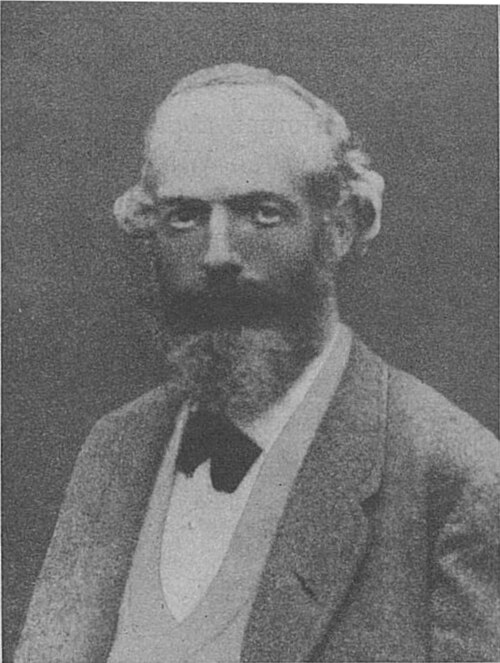
\includegraphics[width=\linewidth]{images/book3/kekule.jpg}
\end{minipage}\hfill
\begin{minipage}[t]{0.74\linewidth}
\vspace{0pt}
1865 年，凯库勒提出苯的六个碳原子构成一个环，
单键与双键交替排列，且很快认为这两种交替极速互换，
以致每个键都完全相同。以 X 射线衍射
测得的等长键与铺展于整个环上的 $\pi$ 轨道，使他的直觉获得了现代形式；
1931 年，\omterm{thm:b2:huckel:huckel-rule}{休克尔规则}解释了为何六个电子（而非四个或
八个）能使环具有特殊性。（肖像，1873 年，作者不详，公有领域，
取自维基共享资源。）
\end{minipage}
\end{history}

\section{共轭体系与光}

\begin{proposition}[多烯的能隙]\label{prop:b2:huckel:gap}
对线性多烯，设其碳原子数为 $n$（$n$ 为偶数），则
最高占据与最低空 $\pi$ 能级之间的能隙为 $4|\beta|\sin(\pi/(2(n + 1)))$：它随
链长增加而减小。
\end{proposition}

\begin{proof}
最高占据能级为 $k = n/2$，最低空能级为 $k = n/2 + 1$。记 $\theta_k =
k\pi/(n + 1)$，则 $E_{n/2+1} - E_{n/2} = 2|\beta|(\cos\theta_{n/2} - \cos\theta_{n/2+1}) = 4|\beta|
\sin\frac{\theta_{n/2} + \theta_{n/2+1}}{2}\sin\frac{\theta_{n/2+1} - \theta_{n/2}}{2}$，而第一个正弦
为 $\sin(\pi/2) = 1$。它随 $n$ 增大而减小，因 $\sin$ 在
$[0, \pi/2]$ 上递增。
\end{proof}

\begin{omfigure}
\begin{tikzpicture}
\begin{axis}[width=0.5\linewidth, height=5cm, xmin=0, xmax=22, ymin=0, ymax=2.2,
  axis x line=bottom, axis y line=left, xlabel={碳原子数 $n$}, ylabel={能隙$/|\beta|$},
  tick label style={font=\small}, label style={font=\small}]
\addplot[omThm, thick, mark=*, mark size=1.3pt] table[x=n, y=gap] {figdata/out/bachelor-2-huckel-b.dat};
\end{axis}
\end{tikzpicture}\hfill
\begin{tikzpicture}
\begin{axis}[width=0.48\linewidth, height=5.4cm, xmin=-1, xmax=11, ymin=-2.4, ymax=2.4,
  axis x line=none, axis y line=left, ylabel={$(E - \alpha)/|\beta|$}, clip=false,
  tick label style={font=\small}, label style={font=\small}]
\addplot[only marks, mark=-, mark size=5pt, very thick, omDef] table[x=x, y=e] {figdata/out/bachelor-2-huckel-a.dat};
\draw[densely dotted] (axis cs:-1,0) -- (axis cs:11,0);
\node[anchor=north, font=\scriptsize] at (axis cs:0,-2.45) {C$_2$};
\node[anchor=north, font=\scriptsize] at (axis cs:2,-2.45) {C$_3$};
\node[anchor=north, font=\scriptsize] at (axis cs:4,-2.45) {C$_4$};
\node[anchor=north, font=\scriptsize] at (axis cs:6,-2.45) {C$_6$};
\node[anchor=north, font=\scriptsize] at (axis cs:8,-2.45) {四元环};
\node[anchor=north, font=\scriptsize] at (axis cs:10,-2.45) {六元环};
\end{axis}
\end{tikzpicture}

{\small 左图：线性多烯的休克尔能隙随链长增加而减小，这正是长共轭链
吸收波长更长的光、乃至可见光的原因。
右图：乙烯、烯丙基、丁二烯、己三烯（链状）以及
环丁二烯、苯（环状）的计算能级；成键能级位于 $\alpha$ 以下。}
\end{omfigure}

引入杂原子时，需改变其\omterm{def:b2:diatomic-mos:integrals}{库仑积分} $\alpha_X = \alpha + h\beta$，并改变与之相连键的
\omterm{def:b2:diatomic-mos:integrals}{共振积分}。这是一个含可调参数的模型，它保留了定性结论
（电负性较强的原子，$h > 0$，会把 $\pi$ 电子密度拉向自身），
但其数值是拟合得到的，而非推导得到的。

\section{练习}

\begin{exercise}[$\star$]\label{exo:b2:huckel:1}
求烯丙基阳离子、自由基和阴离子的 $E_\pi$。
\end{exercise}

\begin{exercise}[$\star$]\label{exo:b2:huckel:2}
计算丁二烯的 $E_\pi$，所用能级为 $\alpha \pm 1.618\beta$、$\alpha \pm 0.618\beta$。
\end{exercise}

\begin{exercise}[$\star$]\label{exo:b2:huckel:3}
判断下列物质是\omterm{def:b2:huckel:aromatic}{芳香性的}、\omterm{def:b2:huckel:aromatic}{反芳香性的}还是两者皆非（若为平面结构）：苯、环戊二烯基阴离子、
环戊二烯基阳离子、环庚三烯正阳离子 \ce{C7H7+}、环丁二烯、平面
环辛四烯。
\end{exercise}

\begin{exercise}[$\star$]\label{exo:b2:huckel:4}
画出平面环辛四烯的弗罗斯特圆，并将其 8 个 $\pi$ 电子填入其中。
\end{exercise}

\begin{exercise}[$\star\star$]\label{exo:b2:huckel:5}
计算丁二烯的\omterm{def:b2:huckel:delocalisation}{离域能}，并以 \unit{kJ/mol} 为单位给出，取
$|\beta| = \qty{75}{kJ/mol}$。与环己-1,3-二烯催化氢化数据中的
\qty{10}{kJ/mol} 相比较。
\end{exercise}

\begin{exercise}[$\star\star$]\label{exo:b2:huckel:6}
计算丁二烯的 $\pi$ \omterm{def:b2:diatomic-mos:bond-order}{键级}，并预测其 C--C 键中哪一根
最短。
\end{exercise}

\begin{exercise}[$\star\star$]\label{exo:b2:huckel:7}
五元环的能级为 $\alpha + 2\beta$、$\alpha + 0.618\beta$（二重简并），
$\alpha - 1.618\beta$（二重简并）。分别为环戊二烯基阴离子和
阳离子填入电子，并比较二者。
\end{exercise}

\begin{exercise}[$\star\star$]\label{exo:b2:huckel:8}
利用七元环的能级，解释为何环庚三烯基溴
表现出盐的性质，即溴化环庚三烯正。
\end{exercise}

\begin{exercise}[$\star\star$]\label{exo:b2:huckel:9}
检验己三烯的迹规则，其能级为 $\alpha \pm 1.802\beta$、$\alpha \pm
1.247\beta$、$\alpha \pm 0.445\beta$。
\end{exercise}

\begin{exercise}[$\star\star\star$]\label{exo:b2:huckel:10}
由闭式推导己三烯的能级及其\omterm{def:b2:huckel:delocalisation}{离域能}。
\end{exercise}

\begin{exercise}[$\star\star\star$]\label{exo:b2:huckel:11}
若环丁二烯为正方形，则将有两个未成对电子。解释真实分子
为何呈长方形，具有两根短键和两根长键。
\end{exercise}

\begin{exercise}[$\star\star\star$]\label{exo:b2:huckel:12}
在双原子 $\pi$ 体系 \ce{C=X} 中，取 $\alpha_X = \alpha + \beta$（模型值，$h = 1$），且
$\beta_{\ce{CX}} = \beta$，求两个能级，以及在两个电子占据下
C 与 X 上的 $\pi$ 电荷。
\end{exercise}

\section{周末问题：苯缺失的能量}

\begin{problem}[{周末问题——由催化氢化焓求苯的芳香稳定化，苯的
休克尔能级及其离域能，$|\beta|$ 的取值，以及
与己三烯和
环辛四烯的比较}]
\label{pb:b2:huckel:1}
数据：气态物质的生成焓（\unit{kJ/mol}）：苯 82.9、
环己-1,3-二烯 104.6、环己烯 $-4.3$、环己烷 $-123.1$。键长
（pm）：苯 139.7、乙烯 133.9、乙烷 153.6。
% ledger: dfh:C6H6_g, dfh:C6H8_g, dfh:C6H10_g, dfh:C6H12_g, geo:C6H6.rCC, geo:C2H4.rCC, geo:C2H6.rCC

\medskip
\noindent\textbf{第一部分——催化氢化。}
\begin{enumerate}
  \item 计算环己烯催化氢化为环己烷的 $\Delta_r H^\circ$。
  \item 对环己-1,3-二烯同样计算。
  \item 对苯同样计算。
  \item 三个相互独立的双键催化氢化时将释放多少热量？
  \item 由此推出苯的稳定化能。
  \item 与共轭二烯的稳定化能相比较，并加以评论。
\end{enumerate}

\medskip
\noindent\textbf{第二部分——苯的\omterm{def:b2:huckel:method}{休克尔方法}。}
\begin{enumerate}[resume]
  \item 写出苯的休克尔矩阵。
  \item 由环状公式求出其能级。
  \item 将 6 个 $\pi$ 电子填入这些能级。
  \item 计算 $E_\pi$。
  \item 计算三个孤立双键的 $E_\pi$。
  \item 由此得出\omterm{def:b2:huckel:delocalisation}{离域能}。
  \item 检验迹规则。
\end{enumerate}

\medskip
\noindent\textbf{第三部分——$|\beta|$ 的取值。}
\begin{enumerate}[resume]
  \item 令\omterm{def:b2:huckel:delocalisation}{离域能}与第一部分所得的稳定化能相等，并求出
        $|\beta|$。
  \item 取该值，预测丁二烯的\omterm{def:b2:huckel:delocalisation}{离域能}，并与
        第一部分的结果相比较。
  \item 计算苯的 $\pi$ \omterm{def:b2:diatomic-mos:bond-order}{键级}。
  \item 将其与丁二烯的\omterm{def:b2:diatomic-mos:bond-order}{键级}相比较。
  \item 解释苯的键长为何相等，并说明它们落在什么范围内。
\end{enumerate}

\medskip
\noindent\textbf{第四部分——其他环与链。}
\begin{enumerate}[resume]
  \item 计算己三烯的\omterm{def:b2:huckel:delocalisation}{离域能}，并与苯进行比较。
  \item 给出平面环辛四烯的能级。
  \item 将 8 个电子填入这些能级：有何问题？
  \item 真实分子如何规避这一问题？
  \item 环丁二烯的情况如何？
  \item 叙述\omterm{thm:b2:huckel:huckel-rule}{休克尔规则}。
  \item 给出 $|\beta|$ 的值，该值由使苯的\omterm{def:b2:huckel:delocalisation}{离域能}
        与其实测稳定化能相匹配而得。
\end{enumerate}
\end{problem}
